\documentclass[11pt,a4paper]{article}
\usepackage[T1]{fontenc}
\usepackage[utf8]{inputenc}
\usepackage[french]{babel}
\usepackage{lmodern}
\usepackage[margin=2.2cm,headheight=15pt]{geometry}
\usepackage[table]{xcolor}
\usepackage{graphicx}
\usepackage{booktabs}
\usepackage{tabularx}
\usepackage{fancyhdr}
\usepackage{microtype}

\definecolor{HeartTeal}{HTML}{087C78}
\definecolor{HeartNavy}{HTML}{16324F}
\definecolor{HeartCoral}{HTML}{EF6A55}
\definecolor{SoftMint}{HTML}{EAF5F3}
\definecolor{SoftGray}{HTML}{F3F5F7}

\pagestyle{fancy}
\fancyhf{}
\lhead{\textcolor{HeartTeal}{\small Rapport de traitement ECG}}
\rhead{\textcolor{HeartNavy}{\small Enregistrement \#1}}
\cfoot{\textcolor{gray}{\thepage}}
\renewcommand{\headrulewidth}{0.4pt}
\renewcommand{\headrule}{\hbox to\headwidth{\color{HeartTeal}\leaders\hrule height \headrulewidth\hfill}}
\setlength{\parindent}{0pt}
\setlength{\parskip}{0.65em}

\begin{document}

\begin{center}
\colorbox{HeartNavy}{%
  \begin{minipage}{0.92\textwidth}
    \vspace{0.55cm}
    \centering
    {\color{white}\Large\bfseries RAPPORT DE TRAITEMENT ECG}\\[0.3cm]
    {\color{white}\LARGE\bfseries Record 1}\\[0.25cm]
    {\color{white!80}\large Filtre passe-bande Butterworth
      \textcolor{HeartCoral}{\bfseries 0.5--40 Hz}
      \quad|\quad ordre 4}\\
    \vspace{0.55cm}
  \end{minipage}%
}
\end{center}

\vspace{0.25cm}
\color{HeartTeal}\rule{\textwidth}{1.2pt}
\color{black}

\section*{\textcolor{HeartNavy}{Comparaison du signal}}
La figure ci-dessous compare l'enregistrement ECG brut au signal après
filtrage passe-bande. Le filtrage est appliqué en phase nulle afin de
préserver l'alignement temporel des événements du signal.

\begin{figure}[ht]
  \centering
  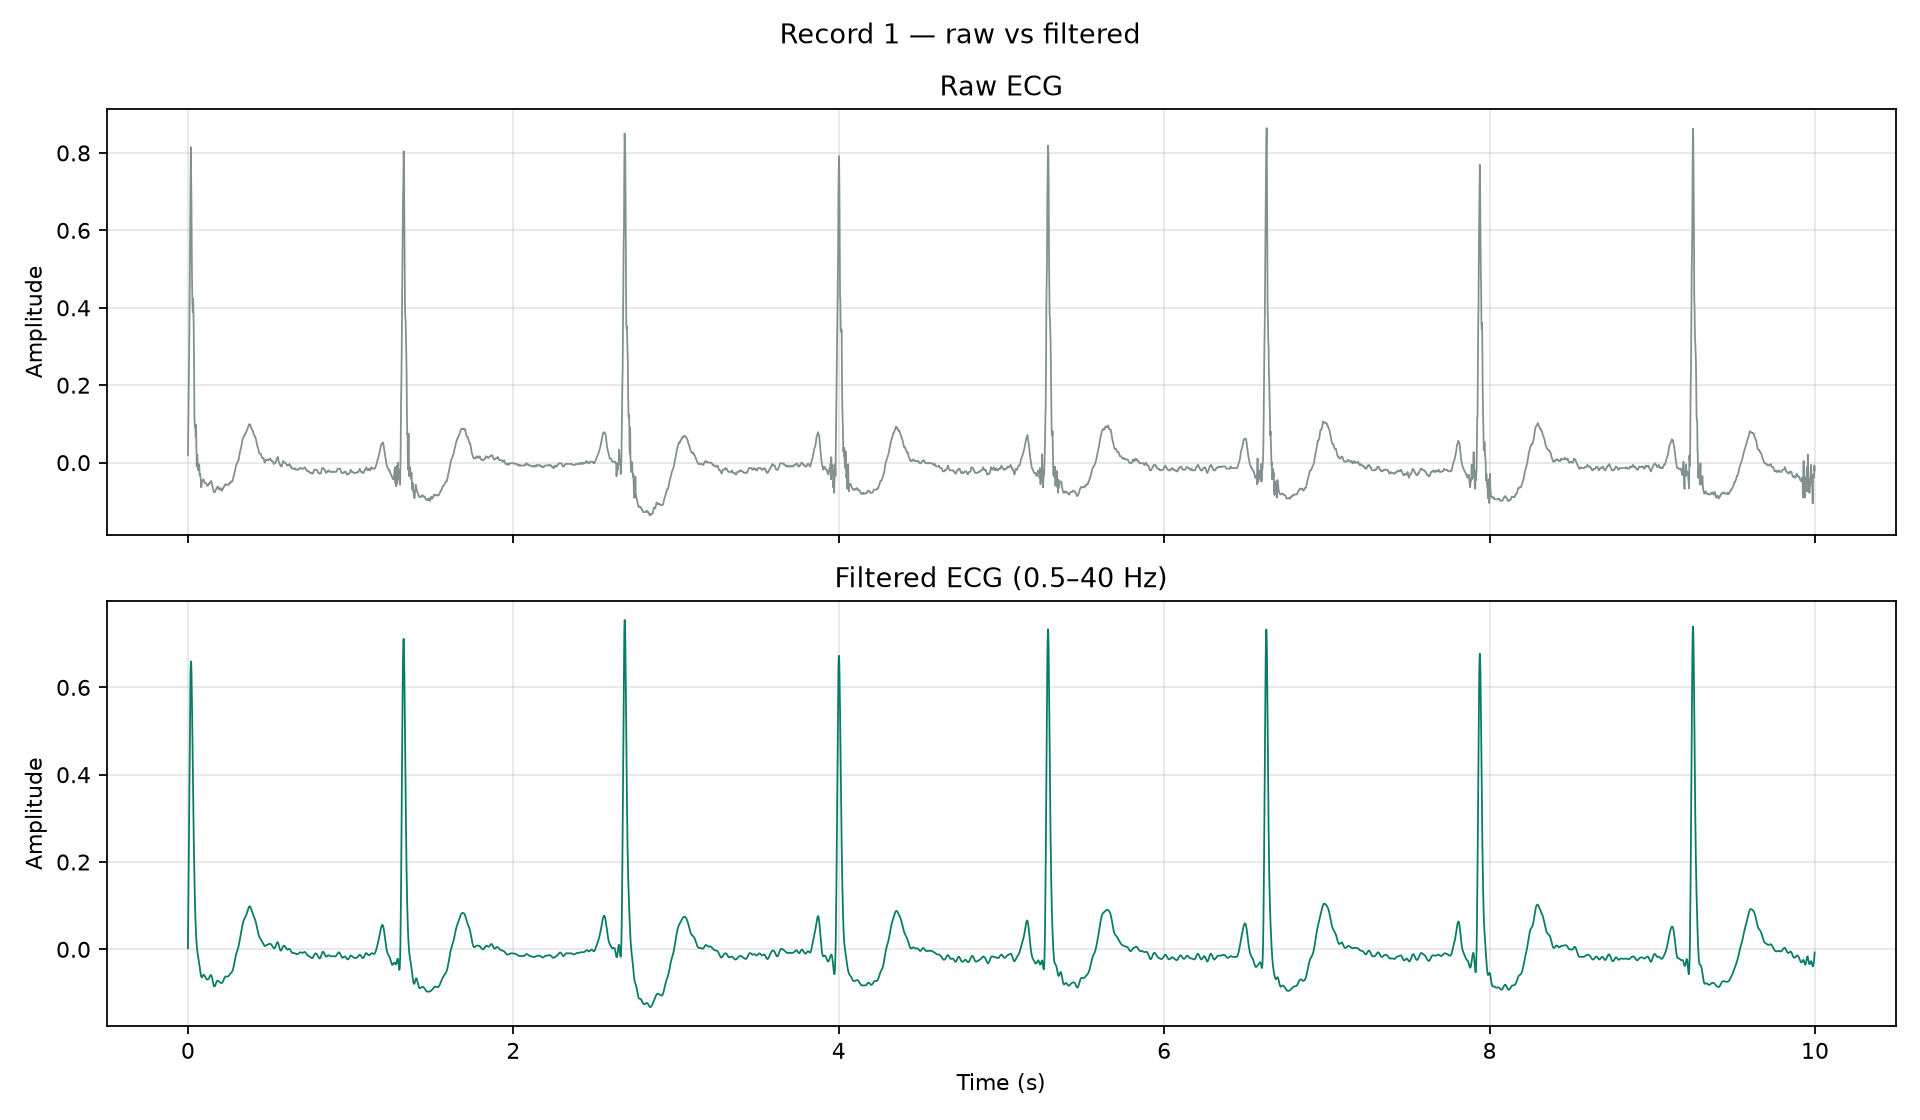
\includegraphics[width=\textwidth,height=0.58\textheight,keepaspectratio]{record-1-comparison.png}
  \caption{Comparaison des signaux brut et filtré pour
    \textbf{Record 1}.}
\end{figure}

\section*{\textcolor{HeartNavy}{Paramètres de l'analyse}}
\rowcolors{2}{SoftGray}{white}
\begin{tabularx}{\textwidth}{>{\bfseries}X r}
\rowcolor{SoftMint}
\textcolor{HeartNavy}{Métrique} & \textcolor{HeartNavy}{Valeur}\\
Fréquence d'échantillonnage & 500 Hz\\
Nombre d'échantillons & 5000\\
Ordre du filtre Butterworth & 4\\
Bande passante & 0.5--40 Hz\\
\bottomrule
\end{tabularx}

\vfill
{\small\color{gray}Traitement numérique réalisé avec un filtre Butterworth
à phase nulle (\texttt{scipy.signal.sosfiltfilt}).}

\end{document}
